\section{Literature Review}
\subsection{Abell 2162}
Giacintucci et al. (2013) presented the morphological study and spectral analysis for sample of 13 cD galaxies in rich and poor clusters of galaxies. Their study is based on new high sensitivity Gaint Meterwave Radio Telescope (GMRT) observations at 1.28 GHz, 610 MHz and 235 MHz. The GMRT full resolution image at 235 MHz shows two opposite lobes, with lack of a central compact component at both frequencies. The radio emission is weak and surface brightness is low. A similar double morphology without central component was found also at 1.4 GHz by Owen \& Ledlow (1997). The source has linear size of $\approx$ 90 $\times$ 38 Kpc. They also found that A2162 shows fairly relaxed morphology of the lobes and lack nuclear emission and these features are consistent with the idea that they are aged radio galaxies.\\\\
Liuzzo et al. (2010) presented new VLBI observations at 5GHz of a complete sample of Brightest Cluster Galaxies (BCGs) in Abell Clusters. The detailed discussion about the distribution of the absolute magnitude of BCGs which is not correlated to the dynamic equilibrium of their host-clusters can be found in Hoessel et al. (1980). These galaxies are intimately related to the collapse and formation of clusters: recent models suggest that BCGs must form earlier, and the galaxy merging with the clusters during collapse within a cosmological hierarchy is a visible scenario (Bernardi et al. 2006). The Abell cluster is a low X-ray luminosity clusters (Burns  et al. 1994). Its BCG is NGC6086 is a bright cD galaxy which hosts a double-lobed radio source. In the NVSS image, the total flux density is $\approx$ 108.7 nJy. The radio spectrum and morphology suggests that it is relic galaxy where the core radio activity stopped some time ago.\\\\
Abell 2162 is member of the Hercules super cluster complex (Einasto et al. 2001). The X-ray emission of this nearby cluster of galaxies has been studied by Ledlow et al. (2003) who reported an X-ray luminosity in the 0.5-2.0 keV band of 0.16 $\times 10^{43}$ erg\,s$^{-1}$ based on ROSAT data. The fading radio lobes of B2 1610+29 associated with NGC 6086, the brightest galaxy of the cluster located close to the X-ray peak.\\\\
Donzelli, Muriel, Madrid (2011) derived detailed R band luminosity profiles and light profiles were initially fitted with a Sersic's $R^{\frac{1}{n}}$ model. The effective surface magnitude and central surface magnitude is 20.85 and 22.46 respectively. The effective radius is 7.19 Kpc and n parameter is 3.92.\\\\
Gal et al. (2000) presents photometric redshifts for 431 Abell clusters imaged as part of the Palomar Abell Cluster Optical Survey (PACOS). For this cluster (\textit{g-r}) is 0.43867 and $g_{mean}$ = 20.2053.\\\\
Miller (2001) used the NRAO VAL Sky Survey (NVSS) to identify radio galaxies in eighteen nearby Abell clusters. A2162 contains only four radio galaxies consitent with the cluster at \textit{z} $\approx$ 0.03 whereas six radio galaxies are at \textit{z} $\approx$ 0. The zero point magnitude assumed for POSS II photometry of the cluster is 30.24 and average extinction assumed for POSS II photometry is 0.04. The separation between optical position and radio position as specified in NVSS catalog 29.2 and Radio flux at 1.4 GHz determined directly from the NVSS image 113.4.\\\\
Mahdavi et al. (2001) demonstrated that individual elliptical galaxies and clusters of galaxies form a continuous X-ray luminosity -velocity dispersion($L_X-\sigma$) relation. Their sample of 280 clusters have $L_x\propto\sigma^{4.4}$. For this cluster log$\sigma$ is 2.56$\pm$0.07 km\,s$^{-1}$ and log$L_x$ is 43.32$\pm$0.10 $h_{50}^{-2} $erg\,s$^{-1}$\\\\
Haynes et al. (2004) conducted a study of optical and HI properties of spiral galaxies (size, luminosity, H$\alpha$ flux distribution, circular velocity, HI gas mass) to explore the role of gas stripping as a driver of morphological evolution of clusters. The X-ray temperature of Abell 2162 is 0.9 keV and this is derived from the velocity dispersion. The bolometric luminosity of X-ray is 42.95 erg\,s$^{-1}$. The peculiar velocity, taken from Giovanelli et al. (1997) is 323 km\,s$^{-1}$.\\\\
Ruiter et al. (2008) presented a study of the optical brightness profiles of early type galaxies, using a number of a samples of a radio galaxies and optically selected elliptical galaxies. They collected data from Faber et al. and Laine et al. and found that the optical magnitude of Abell 2162 is -22.75 and  log(P$_t$/WHz$^{-1}$) at 1.4 GHz is 23.26.\\\\
Robinson et al. (2008) determined mass of A2162 is 520.0 M$_\odot$ and the classical radius is 8. The velocity determined from CMB is 9794.4 km\,s$^{-1}$ but the observed velocity is 9689 km\,s$^{-1}$.\\\\
Fritsch and Buchert (1998) discussed implication of the fundamental plane parameters of clusters of galaxies derived from combined optical and X-ray data of a sample of 78 nearby clusters. The optical luminosity of A2162 is 61.319 [$10^{10}L_\odot$] and X-ray luminosity is 0.091 [$10^{44}$\,erg\,s$^{-1}$]. The optical half-light radius of A2162 is 0.530 Mpc.\\\\
Carter et al. (2008) present kinematic parameters and absorption line strength for three brightest cluster galaxies. They have described A2162 as poor cluster or compact group.\\\\
Lauer and Postman (1994) measured the velocity of the Local Group with respect to an inertial frame defined by the 119 Abell and Abell, Corwin \& Olowin (ACO) clusters contained within 15000 km\,s$^{-1}$. Parameter subscript refer to the CMB frame (C), the local Group at rest with respect to the ACIF (L), and the frame implied by recovery of the local Group motion (L), with respect to the ACIF (F). For Abell 2162 $M_c=-22.594$, $M_l=-22.604$ and $M_F=-22.475$.\\\\
West (1989) generated a catlog of 48 probable supercluster  by means of percolation technique using a large sample of Abell clusters with measured redshifts \textit{z} $\leq$ 0.1 and various properties of these superclusters were examined. The orientation of clusters within these supercluster were also examined. Position angle data for clusters have been gathered from many sources in the literature and supplemented with new measurement presented in this paper. (SP=Struble and Peebles 1985, B=Bingeli 1982, D=Struble 1987 (he presents position angle determination for various surface brightness isophotes of first-ranked galxies); J=Tuker and Peterson 1988). The position angle of this abell cluster is 6, 0[SP], 1[B], 179[D], 7[J]. The final value predicted in this paper is 0.\\\\
Struble and Rood (1991) presented a list of redshifts for 758 Abell clusters and velocity dispersion for 121. They also presented another list of 33 Abell clusters with published redshifts, most of which are probably redshifts of foreground or background galaxies superposed on, or near the Abell clusters. In their paper the adopted $z_{adp}= 0.0320$ for this cluster and this was calculated using 5 galaxies. The velocity dispersion $\sigma_{adp}=323$ km\,s$^{-1}$.\\\\
Plionis, Barrow and Frenk (1991) identified a large number of galaxy clusters in the Lick map using an algorithm based on an overdensity criterion. The resulting catlogues contain $\approx$ 6000 clusters out of which 753 is Abell clusters. They determined ellipticities and position angle using Lick map. The mean ellipticity of Abell 2162 (identified at 3.6 level) is 0.301. The position angle determined from the Lick map is 1.7$\pm$10 using 3 overdensity thresholds to define the mean position angle. The value of position angle given by Sruble and Peebles (1985) is 0.\\\\
Henriksen (1992) used the available X-ray data to investigate systematic errors in a complete subsample of the Abell catalog which has been used in studies of large-scale structures. The catalogue of Rich Clusters of Galaxies identified by Abell (1958) contains 2712 entries and these cluster were classified by richness (0-5). The Abell 2162 was studied by Einstein telescope and found the luminosity to be $L_x=0.84\times 10^{43}$ erg\,s$^{-1}$. And the richness of this cluster is 0. It is BM type II-III and RS is Is.\\\\
Postman et al. (1992) have acquired redshifts for a complete sample of 351 Abell clusters with tenth-ranked galaxy magnitude ($m_{10}$) less than or equal to 16.5, including 115 entirely new cluster redshifts. The richness and distance class of Abell 2162 is 0 and 1 respectively. The $m_{10}$ is 13.70 and observed redshift of this cluster is 0.0318 for A2162.\\\\
Wise et al. (1993) had analyzed IRAS image data using a random position, multiple-aperture photometry method to study diffuse far-infrared emission for a sample of 56 clusters of galaxies at 60 and 100 $\mu$m. The radius of A2162 in arcminutes is 57 and log $L_x$=42.86 erg\,s$^{-1}$. This cluster is low-luminosity X-ray clusters.\\\\
Abell (1957) prepared catlogue of 2712 rich cluster of galaxies found on the National Geographic Society-Palmor Observatory Sky Survey. From this catalogue, 1682 clusters are selected to meet specific crietria for inclusion in a homogenous statistical sample. Some criteria to be clusters are richness criterion, compactness criterion, distance criterion, galactic latitude criterion. The richness group is from 0 to 5 which includes count of galaxies 30-49, 50-79, 80-129, 130-199, 200-299, $\geq 300$ respectively. The distance group interval is from 1-7 which inludes the tenth brightest member magnitude is 13.3-14.0, 14.1-14.8, 14.9-15.6, 15.7-16.4, 16.5-17.2, 17.3-18.0 and $\geq 18$. The magnitude of Abell 2162 is 13.7 , richness is 0 and distance is 1.\\\\
White (1978) presented the result of an extensive survey of a wide range of Abell and poor, non-Abell clusters of galaxies. The cluster are classified on a modified Bautz-Morgan system which includes detailed Yerkes form-types and relative brightness of the inner, brighter member galaxies of the cluster, and which is applicable to a wider variety of cluster and group of galaxies than the orginal Bautz-Morgan system. Abell 2162 has distance class 1 and richness class 0. It has $M_{10}=$13.8 and is BM type III. Its abell radius is 64 and central density estimate is I (Intermediate).\\\\
Fanti et al. (1981) carried out survey of 61 abell clusters included in the HEAO-2 satellite observing program was carried out at 1.4 GHz with the Westerbork Synthesis Radio Telescope. In this paper, they presented nine clusters of distance class 1 and 2 and make statistical consideration about the radio emission and structure of the cluster galaxies. Abell 2162 has distance class 1 and richness class 0. The heliocentric mean velocity of the cluster is 9585 km\,s$^{-1}$. It is BM type III and dominant galaxy type in this cluster is Spiral. In this cluster they identified three radio sources. This cluster belongs to a large supercluster including: A2197 and A2199 at $\delta\approx 40^\circ$, the Hercules completed at $\delta\approx 16^\circ$ and some other smaller galaxy groups at intermediate declinations (Ekers et al. 1978, Chincarini et al. 1981). It is at the center of a wide area where secondary consideration, Butcher and Oemler (1978) judge its inclusion in the Abell catalogue as ``a mistake". Out of six galaxies with measured velocity, two have v=15000\,km\,s$^{-1}$, indicating a contamination from back-ground galaxies. Also, evidence of the presence of hot gas in various locations within the supercluster has been pointed out by several author (Jaffe \& Perola 1974, Ekers et al. 1978, Valentijn 1979).
\subsection{Abell 1139}
Sun et al. (2008) presented a systematic analysis of 43 nearby galaxy groups (kT$_{500}=0.7-2.7$ keV or M$_{500}=10^{13}-10^{14}h^{-1}$M$_{\odot}$, $0.012<z<0.12$), based on Chandra archival data. A1139 is the faintest in 2-3 keV system. The redshift extracted from NASA/IPAC Extragalactic Database is 0.0398 and the luminosity distance derived from this redshift is 169. 2MASS $K_s$ band luminosity in terms of log($L_{Ks}/L_{\odot}$) is 11.50 and 1.4 GHz luminosity in log($L_{1.4\text{GHz}}${W Hz}$^{-1}$) from the NRAO VLA Sky Survey (NVSS) or the Sydney University Molonglo Sky Survey (SUMSS), assuming a spectral index of -0.8 is 23.16. Temperature of the hotter component of local soft CXB is 0.25 and the observed flux of the local soft CXB (in unit of $10^{-12}$ ergs cm$^{-2}$\,s$^{-1}$\,deg$^{-2}$) in 0.47-1.21\,keV is $2.6^{+0.4}_{-0.5}$.\\\\
Holden et al. (2009)  compiled a sample of early type cluster galaxies from $0<z<1.3$ and measured the evolution of their ellipticity distribution. For $z<0.05$ sample is selected from Abell cluster in SDSS fifth Data Release (McCarty et al. 2007, SDSS DR5). The redshift of Abell 1139 is 0.0383 (Struble \& Rood 1999). They calculated $R_{200}$ using the formula given in Calberg et al. 1997. In Abell 1139 the velocity dispersion is 436 km\,s$^{-1}$ (Poggianti et al. 2006). The calculated value of $R_{200}$ is 0.67 Mpc and found the number of early type galaxies within $R_{200}$ to be 23.\\\\
Dong, Rasmussen and Mulchaey (2010) performed search for X-ray cavities in hot gas of 51 galaxy groups with Chandra archival data. The cavities were identified based on two method: subtracting an elliptical $\beta$- model fitted to the X-ray brightness, and performing unsharp masking. They found tight correlations between the radial and tangential radii of the cavities and between their size and projected distance from group center, in quantitative agreement with the case for more massive clusters. They suggests that similar physical process are responsible for cavity evolution and disruption in systems covering a large range in total mass. Abell 1139  has no detectable cavities and number of 0.3-2 keV photons from diffuse emission on the central CCD is 1948. The radio luminosity at 1.4 GHz of any radio source within the central bright group galaxy, extracted from the NRAO VLA Sky Survey (Condon et al. 1998) is less than 22.09 W\,Hz$^{-1}$.\\\\
Wojtak and Lokas (2010) analyzed kinematic data of 41 nearby ($z<0.1$) relaxed galaxy clusters in terms of the projected phase-space density using phenomenological, fully anisotriopic model of distribution function. They apply Markov Chain Monte Carlo approach to place constraints on the total mass distribution approximated by the universal NFW profile and the profile of the anisotrypy of galaxy orbits. The  Abell 1139 is BM III type cluster and no thing can be said about the cool core as judged on the basis of Hudson et al. (2010), Chen et al. (2007), White (2000), Jones and Forman (1997). The mass and radius parameter used in their analysis of Abell 1139 is $0.41^{+0.12}_{-0.05}10^{14}$ M$_{\odot}$ and $0.39^{+0.13}_{-0.08}$ Mpc. The viralized mass of this cluster is $4.10^{+0.39}_{-0.36}$ and the concentration parameter is $3.53^{+0.51}_{-1.25}$. The ratio of the radial velocity dispersion and the tangential velocity dispersion at the cluster center and viral radius is $0.87^{+.28}_{-0.19}$ and $1.75^{+0.22}_{-0.28}$ respectively. The anisotropy at the cluster center and virial radius is $-0.31^{+0.56}_{-0.83}$ and $0.67^{+0.07}_{-0.14}$ respectively. In their study the virial mass of the clusters correlates very well with the velocity dispersion, the X-ray temperature and the X-ray luminosity of the clusters.\\\\
Harrison et al. (2010) presented a catlogue of galaxies well suited to the investigation of the early type galaxy formation and evoluiton. A1139 has velocity dispersion of $504\pm 47$ km\,s$^{-1}$ and the total number of galaxies used to calculate the red shift of $0.0396\pm 0.0002$ is 106 and it is B-M III cluster.\\\\
Poggianti et al. (2004) studied how the proportion of star-forming galaxies evolves as a function of galaxy environment, using the [$O_{II}$] line in emission as a signature of ongoing star formaion. In their study they used 10 galaxies of Abell 1139 to find its [$O_{II}$] fraction. They also calculated $R_{200}$ to be 1.06 Mpc. The value of [$O_{II}$] fraction corrected for completeness and uncorrected for completeness are $0.38\pm0.20$ and 0.40 respectively.\\\\
Popesso et al. (2008) considerd a large sample of optically selected clusters, in order to elucidate the physical reason for the existence of X-ray underluminous clusters. For this purpose they analyze the correlation of X-ray and optical properties of a sample of 137 spectroscopically confirmed abell clusters in SDSS database. They used the properties extracted from the SDSS DR3 paper. According to this paper, Abell 1139 has 89 cluster members within 1 Abell radius. The cluster red shift is 0.0395 and the velocity dispersion is 376$\pm$34. The mass of the cluster within $r_{200}$ is 1.68 $\times 10^{14}$M$_{\odot}$. The virial radius of the cluster is 1.2 Mpc. Optical luminosity of the cluster is (1.16$\pm$0.25)$\times 10^{12}$ L$_{\odot}$ and the X-ray luminosity in the ROSAT energy band (0.1 - 2.4 erg\,s$^{-1}$) is 0.136$\times 10^{44}$\,erg\,s$^{-1}$. The Dressler \& Shectman Probablity that the cluster doesn't contain substructre is 0.24. This cluster is normal X-ray emitting cluster.\\\\
McDonald et al. (2011) presented the result of a combined X-ray and $H\alpha$ study of 10 galaxy and 17 galaxy clusters using Chandra X-ray Observatory and Maryland Magellan Tunable Filter. They find no difference in morphology or detection frequency of H$\alpha$ filament in group versus clusters over the mass range $10^{13}\,<$\,M$_{500}\,<10^{15}$\,M$_{\odot}$. The value of E(B-V) of A1139 is 0.031 and according to  Sun et al. (2009) the temperature of X-ray at $r_{2500}$, kT= 2.2.\\\\
Donzelli et al. (2011) derived detailed R-band luminosity profiles and structural parameters for a total of 430 brightest cluster galaxies, down to a limiting surface brightness of 24.5 mag\,arcsec$^{-2}$. Light profiles were fittled with Sersic's $R^{\frac{1}{n}}$ model also the logarithmic slope of the metric luminosity $\alpha$ was determined. The effective surface magnitude of A1139 is 21.39 and the effective radius is 6.74 kpc. The n parameter of this cluster is 4.38. The central surface magnitude is 22.45 and the scale length is 22.60 Kpc. The Sersic absolute magnitude and exponential absolute magnitude is -22.92 and -22.99   respectively. The total absolute magnitude is -23.71 whereas the ratio of Sersic to exponential magnitude is 0.93. The $\alpha$ parameter is 0.57. The inner and outer ellipticity is 0.06 and 0.32 respectively. The inner and outer position angle is -51.2 and -82.0 respectively. The metric absolute magnitude is -22.55.   \\\\
Hilton et al. (2013) has combined two data base ROSAT-ESO flux limited X-ray (REFLEX) galaxy cluster survey and 2dF Galaxy Redshift Survey (2dFGRS) survey to study the effect of the large scale cluster environment, as traced by X-ray luminoisity, on the properites of cluster member galaxies. $R_{200}$ calculated taking the $\sigma$= 550$\pm$50 km\,s$^{-1}$ and red shift 0.0396 is 1.3 Mpc. The X-ray luminosity of this cluster in 0.1-2.4 keV is 0.089$\pm$0.018$\times 10^{44}$\,erg\,s$^{-1}$. The completeness of this cluster is 0.90.\\\\
Burgett et al. (2008) carried out one, two and three dimensional tests for detecting the presence of substructure in clusters of galaxies obtained from the 2dF Galaxy Redshift Survey. The sample of 25 clusters used in this study includes 16 clusters not previously investigated for sub-structure. At least three clusters (A1139, A1663, AS333) exhibit velocity-position characteristics consistent with the presence of possible cluster rotation, shear or infall dynamics. The number of galaxies in A1139 is 109 and the proper distances $d_{p}(t_e)$=162 and $d_p(t_0)$=171 given in h$^{-1}$\,Mpc. The richness of A1139 according to Abell, Corwin \& Olowin 1989 is 0 and according to 2dFGR is less than 0. The analysis of A1139 done is based on 106 galaxies. The fitted optical core radius is 0.26 h$^{-1}$\,Mpc with central density of 138 which is fairly typical of the poor clusters in the sample. At large radii the ellipticity is low, $\sim$ 0.2 and the position angle is $\sim 65^{\circ}$. The inner part of this cluster is elongated and the ellipticity within 0.75 Mpc is $\approx$ $100^\circ$. The two dimensional test shows no asymmetry but three dimensional test indicates the presence of strong substructure. There exist a velocity gradient across the cluster. The shear seen in the velocity structure may indicate the cluster has a significant rotation. Alternatively, the cluster may be in the late stage of a double merger with two subclumps spiraling in to merge with the main system. The three dimensional tests and the cluster morphology indicate that the cluster is dynamically interesting. However Kriessler \& Beers (1997) and Krywult, MacGillivry \& Flin (1999) concluded that the cluster is unimodal with no substructure while West \& Bothun (1990) found marginal evidence of substructure.\\\\
Ebeling et al. (2008) present low-flux extension of the X-ray selected ROSAT Brightest Cluster Sample (BCS) published in  Paper I series. A1139 has $n_H$ 3.9 $\times 10^{20}$cm$^{-2}$ and the temperature 2.1 keV. The flux of the X-ray in range 0.1-2.4 keV is 4.2$\times 10^{-12}$\,erg\,cm$^{-2}$\,s$^{-1}$ and the luminosity is 0.29$\times 10^{44}$\,erg\,s$^{-1}$.\\\\
Struble and Rood (1999) presented a compilation of redshifts for 1572 Abell, Corwin \& Olowin cluster referenced to both heliocentric and cosmic background radiation reference frames, and 395 velocity dispersions corrected to the reference frame of the cluster. A1139 has the heliocentric redshift 0.0398  and the redshift with respect to cosmic background radiaion derived from $\bar{z_h}$ is 0.0386. The velocity disperson in the rest frame of the cluster is 351 km\,s$^{-1}$. The mass of A2162 is 12307.5 $\times 10^{12}$M$_{\odot}$  and the classical radius is 8. The velocity determined from CMB is 12079.8 km\,s$^{-1}$ but the observed velocity is 11730 km\,s$^{-1}$.\\\\
Krywult, MacGillivray \& Flin (1999) searched the presence of subclustering in 18 rich Abell cluster by the method based on the wavelet transform applied to the position of galaxies. A1139 is type I cluster and has redshift 0.0383 and contains 239 galaxies. Baier (1979, 1983), Baier \& Mai (1977, 1978), Bird (1993), Krywult et al. (1996, Surface number density contour plots), Krywult(1997, symmetry and separation test proposed by West et al. (1988)), West \& Bothun (1990) found no evidence of the subclustering in A1139. Also by applying wavelet analysis of the positional data for galaxies of 18 abell cluster Krywult et al. found A1139 are unimodal, show no evidence of any substructues.\\\\
Willick (1998) presented first result from a Tully-Fisher (TF) survey of the cluster galaxies. The galaxies are drawn from 15 abell clusters that lie in the redshift range $\sim$ 9000-12000\,km\,s$^{-1}$ and are distributed uniformly around celestial sky. A1139 is one of the sample cluster (Las Campanas Clusters) with redshift 0.383 and Abell richness 0 and photographic magnitude of the 10$^{th}$ brightest cluster member is 15.0 (ACO).\\\\
Dale et al. (2008) had obtained I band Tully-Fisher (TF) measurements for 522 late-type galaxies in the fields of 52 rich Abell clusters distributed throughout the sky between $\sim$ 50 and 200h$^{-1}$\,Mpc. They had estimated corrections to the data for various forms of observational bias, most notably cluster population incompleteness bias. The number of cluster members with reliable photometry and velocity widths in A1139 is 11. The cluster offsets from the template zero point $(a_{bias}-a_{tf})$ is -0.17.\\\\
Frithsch and Buchert (1998) discussed the implication of the fundamental plane parameters of clusters of galaxies derived from combined optical and X-ray data of a sample of 78  near by clusters. One of the cluster in their sample is A1139 whose optical luminosity is 123.110 $\times 10^{10}L_{\odot}$ and X-ray luminosity is 0.706 $\times 10^{44}$\,erg\,s$^{-1}$. The optical half-light radii is 1.138 Mpc.\\\\
Dale et al. (1999) presented first result of an all sky observing program designed to improve the quality of I band Tully-Fisher template and to obtain the reflex motion of the Local Group with respect to clusters to $z\sim 0.06$. They have used A1139 as a sample cluster and obtained the helocentric velocity 11855$\pm$59\,km\,s$^{-1}$ and velocity with respect to cosmicmicro backgroud is 12218 km\,s$^{-1}$. The value of V$_x$= -3026\,km\,s$^{-1}$,V$_y$= 10399\,km\,s$^{-1}$ and V$_z$= -5656\,km\,s$^{-1}$. \\\\
Batuski et al. (1991) presented result of fourteen North Galactic Cap Abell clusters that were previously unmeasured. Abell 1139 has distance class 3 and richness class 0. The velocity after eliminating the effect of the motion  of sun and earth is 11490\,km\,s$^{-1}$. The H, K, H$\beta$, Mg, Na lines were used to determine the redshift of this cluster.\\\\
Sandage et al. (1991) calculated $m(r)$ growth curve and the Petrosian $\eta(r)$ curve. A1139 has the redshift of 0.0376 and 1\,094 is the factor by which if we multiply the angular radius we calculate the linear radius in Kpc. f is derived from the redshifts and an assumed $H_0=50$\,km\,s$^{-1}$Mp$^{-1}$. The adopted redshift is from Schombert (1987). So the angular radius is $30.9^{\prime\prime}$ and linear radius is 33.8 Kpc. The total V magnitude from calculated and corrected m$(\infty)$ growth curve is 13.4 and adopted distance modulus from redshift is 36.77. The average effective surface brightness is 22.8 V\,mag\,arcsec$^{-2}$.\\\\
Plionis, Barrow and Frenk (1991) determined the shapes of the galaxy clusters found in projection. They used the Lick map of galaxies as their basic data set which enabled them to identify and analyze a sample clusters which is nearly an order of magnitude larger than those studied previously (Binggeli 1982). The mean ellipticity of Abell 1139 identified at 3.6 level is 0.207.\\\\
Huchra and Geller (1992) acquired redshifts for a complete sample of 351 abell cluster with tenth-ranked galaxy magnidute ($m_{10}$). They used this survey to search for large-scale coherent structures and the distribution of superclusters. Abell 1139 lies in richness class 0 and distance class 3. Its first rank magnitude is 13.80 and tenth rank magnitude is 15.00. The estimated red shift from Leir \& Bergh (1977) is 0.0420 and observed redshift is 0.0397.\\\\
Wise et al. (1993) examined the distribution of far-infrared emission from the cluster as a whole and it is clear from their observation that real flows must be inhomogenous, with a mixture of temperature and densities at given radius. The abell radius of A1139 is 49 arcmin and the common logarithm of X-ray luminosity is 43.47 erg\,s$^{-1}$. The cluster spiral fraction is 55\% and it belongs to class V (Low luminisity x-ray clusters). The IRAS infrared excess in $4^{\prime}$, 10$^{\prime}$, 20$^{\prime}$ and abell radius $r_a$ centered at clusted center in 60$\mu$m is 85, 45, 49, 38, 63 and in 100$\mu$m is 58, 52, 49, 37, 63 respectively.\\\\
Plionis (1994) estimated position angle of large number of Abell and Shectman (Shectman 1985) clusters, identified in the Lick map as surface galaxy-density enhancements. He also determined the major axis orientation of the 202 abell clusters. Abell 1139 also known as Shectman cluster 61 has the position angle 112.5, measured relative to North in the anti-clocksiwe direction and this defines the orientation of the cluster.\\\\
Wu and Han (1994) predicts that the effect of gravitational lensing by the matter associated with cluster of galaxies can magnify background, leading to an enhancement of source number density around foreground cluster of galaxies. They conduct  a search for the association of distant radio-bright quasars with Abell clusters using the 1-Jy and 2-Jy all sky catlogs. Abell 1139 is found to be near the quasar 1055+01 having redshift 0.888. The angular separation is $0.13^{\circ}$.\\\\
\subsection{Abell 2366}
Struble and Rood (1987) presented list of redshifts  for 578 Abell clusters, and velocity dispersion for 77, available as of 1986 July. The redshifts  is 0.542 and in this 1 galaxy was considered. The velocity dispersion is 14 km\,s$^{-1}$.\\\\
Lambas, Groth and Peebles (1988) confirmed that Argyres et al. (1986) result that galaxy count on scale to at least 15 $h^{-1}$Mpc are systematically higher in the direction of the major axes of brightest cluster galaxies using independent sample of brightest galaxies in rich clusters in the southern galactic hemisphere. The abell 2366 has redshift of 0.054 and the postion angle of $115^\circ$.\\\\
Schombert (1988) used single-band photographic and CCD surface photometry to determine luminosity and structural properties of the extended, faint envelopes around 27 cD galaxies. Galaxies classified as cD occupy a special place in the scheme of extragalactic structure by being intermediate in scale between normal galaxies and cluster-sized entities and may be important for tracing the behavior of cluster dynamics (Tonry 1987). Abell 2366 is BM I-III and luminosity of G1 (F) galaxy is log($M_{gal}$)=11.02 and the luminosity of the envelope of this galaxy is log(L$_{env}$)=10.52.\\\\
Baier and Ziener (1989)  presented the compilation of publication with photometeric data in and around clusters of galaxies. Abell 2366 was studied with photographic data by Malumuth (1985), Horbey (1983), Murphy (1983), Schombert (1986), Struble (1987).\\\\
West (1989) generated a catlog of 48 probable supercluster by means of percolation technique using a large sample of the Abell clusters with measured redshifts $z\leq$0.1 and various properties of these supercluster are then examined. They also determined the orientation of clusters within these supercluster. Position angle data for cluster were gathered from many sources. Abell 2366 lies on the supercluster number 19. The position angle is 161 (Struble and Peeble 1985), 115 (Lambas, Groth and Peebles 1988), 143 (Struble 1987, position angle is determined for various surface brightness isophotes of first-ranked galaxies). The average of the position angle is 139$^\circ$  with standard deviation 19$^\circ$.\\\\
Abell, Corwin and Olowin (1989) compiled a all-sky catalog of 4073 rich clusters of galaxies, each having at least 30 members within the magnitude range $m_3$ to $m_3+2$ (m$_3$ is the magnitude of the third brightest cluster member) and each with a nominal redshift less than 0.2. Abell 2366 is BM type I-II cluster (Bautz and Morgan 1970) and the background corrected count of cluster member in magnitude range $m_3$ to $m_3$+2 is 47. The cluster redshift (Struble and Rood, 1987) is 0.0542. The richness and distance class is 0 and 4 respectively (Abell 1958). $m_{10}$ (the red magnitude of tenth brightest cluster ) is 15.9 (Abell 1958).\\\\
Sandage and Perelmuter (1981) obtained petrosian radii, effective radii, apparent magnitude and surface brightness of few ranked galaxies in 56 nearby cluster and groups using data from literature. A2366 has redshift 0.0542 and factor f is 1.577. It is  the factor by which to mutiply the angular radius to calculate the linear radius in kpc. The factor f is derived from the redshift and an assumed Hubble constant of 50 km\,s$^{-1}$Mpc$^{-1}$. The total V magnitude from the calculated and corrected $m(\infty)$ growth curve is 13.4 and adopted distance radius from redshifts is 37.56. The absolute magnitude is -24.2. The measured angular ``effective " radius in arcsecond is $27.5^{\prime\prime}$ and the resulting linear radius obtaining by multiplying $r_e^{\prime\prime}$ by f is 15.4 and the effective surface brightness is  19.8.\\\\
Plionis, Barrow and Frenk (1991) identified a large number of galaxy cluster in the Lick map using algorithm based on an overdensity criterion. The resulting catlogues contain $\sim$ 6000 clusters (with $|b|\geq40^\circ$) out of which 753 are Abell clusters. In this paper they were mainly concerned with the shapes of galaxy clusters found in projection and used the Lick map of galaxies as their basic data set. The  mean ellipticity of Abell cluster A2366 (identified at 3.6 level) is 0.193.\\\\
Postman, Huchra and Geller (1992) acquired redshifts for a complete sample of 351 Abell clusters with tenth ranked galaxy magnitude ($m_{10}$) less than or equal to 16.5. Abell 2366 has richness and distance class 0 and  4 respecively. The first ranked magnitudes and tenth-ranked magnitude are 13.20 and 15.90 respectively. The estimated redshift (Leir \& Bergh 1977) is 0.0600 and observed mean redshift 0.0545 using 2 galaxies.\\\\
Plionis (1994) estimated position angles of a large number of Abell and Schetman clusters, identified in the Lick map as surface galaxy-density enhancements. Abell 2366 also known as Schetman 429 has postion angle 133.6.\\\\
Cox, Bregman and Schombert (1995) examined the frequency with which central dominant galaxies are sources of far-infrared emission in a complete sample of galaxies. But for Abell 2366 they didn't detect anything.\\\\
Struble and Rood (1999) presented a compilation of redshifts for 1572 Abell, Corwin \& Olowin (ACO) clusters, referenced to both the heliocentric and cosmic background radiation reference frames. Abell 2366 which was already listed in Abell (1958) has adopted heliocentric redshifts $(\bar{z}_h)$ 0.0529 and redshift with respect to cosmic background radiation ($\bar{z}_c$) is 0.0517 which is derived from $\bar{z}_h$. The adopted velocity disperion in rest frame of cluster $\sigma_{corr}$ is 490 km\,s$^{-1}$.
\section{Anisotropy in the Polar and Azimuthal Angle Distributions}
In order to compare our observed
$\theta$ and $\phi$-distributions with expected isotropic
distribution curves, we have carried out chi-square,
autocorrelation, Fourier (Godlowski 1993), Kolmogorov-Smirnov
(K-S) (Stephens 1970, Press et al. 1992, Kanji 1995) and Kuiper-V
(Kuiper 1962, Stephens 1970) tests. 
These tests are described in the appendix. These tests are a proper method in our
case, because $\theta$ and $\phi$ are independent data. The
significance level is chosen to be 95\%, the null hypothesis is
established to be an equidistribution for the $\theta$ and $\phi$.
As null hypothesis a spatial isotropy of the angular momentum
vector was chosen. In cases of too small sample size only the K-S
and Kuiper-V tests are meaningful. The conditions for anisotropy
are the following: chi-square probability P$(>\chi^2)$ $<$ 0.050,
auto-correlation coefficient (C/C($\sigma$)) and first order
Fourier coefficient ($\Delta_{11}$/$\sigma$($\Delta_{11}$)) $>$ 1
and Fourier probability P($>\Delta_1$) $<$ 0.150, K-S = 1,
Kuiper-V = 1. In the $\theta$-distribution, a positive (negative)
$\Delta_{11}$ suggests that the spin vectors or angular momentum
vectors of galaxies tend to orient parallel (perpendicular) with
respect to the reference coordinate system. In the
$\phi$-distribution, a positive (negative) $\Delta_{11}$ suggests
that the spin vector projections of galaxies tend to point
radially (tangentially) with respect to center of the reference
coordinate system.
\begin{table*}[h]
\caption[]{Statistics of the polar
($\theta$) and azimuthal angle ($\phi$) distributions of galaxies
in three rotating clusters with respect to galactic (G) and
Supergalactic (S) coordinate systems. The first three columns list
the Abell number, chi-square probability (P$(>\chi^2)$) and
auto-correlation coefficient (C/C($\sigma$)). The next two columns
give the first order Fourier coefficient
$\Delta_{11}$/$\sigma$($\Delta_{11}$) and first order Fourier
probability P($>\Delta_1$). The last two columns list the results
of Kolmogorov-Smirnov (K-S) and Kuiper-V (KV) tests. In these
tests, ``0" denotes that the null hypothesis (isotropy) can not be
rejected at the chosen significance level, ``1" designates that
the null hypothesis can be rejected (anisotropy). }
$$
 \begin{array}{p{0.15\linewidth}ccccccc}
            \hline
            \noalign{\smallskip}
            Cluster  &  $P$(>\chi^2)$$ & $C/C($\sigma$)$  &   $$\Delta_{11}$/$\sigma$($\Delta_{11}$)$  &  $P($>\Delta_1$)$ & $K-S$   &  $Kuiper-V$  \\
                   &  $G$/$S$        &   $G$/$S$        &  $G$/$S$                                   & $G$/$S$           & $G$/$S$ &  $G$/$S$  \\
                   \noalign{\smallskip}
            %\hline
%            position angle(PA)\\
%            \hline
%            A0954   &   0.052/0.129   &   -0.2/+0.2    &   +0.7/+1.0    &   0.707/0.540   &   0/0   &   0/0   \\
%            A1139   &   0.339/0.884   &   -0.0/-0.2    &   -1.3/+0.4    &   0.211/0.921   &   0/0   &   0/0   \\
%            A1399   &   0.404/0.825   &   -0.7/-0.1    &   -0.6/+0.6    &   0.755/0.801   &   0/0   &   0/0   \\
%            A2162   &   0.360/0.484   &   -0.9/-0.4    &   -0.6/+0.5    &   0.787/0.842   &   0/0   &   0/0   \\
%            A2169   &   0.889/0.761   &   -0.0/+0.1    &   +0.0/+0.2    &   0.988/0.966   &   0/0   &   0/0   \\
%            A2366   &   0.598/0.300   &   +0.2/-0.1    &   +0.4/+0.3    &   0.835/0.893   &   0/0   &   0/0   \\
            \hline
            polar angle($\theta$) \\
            \hline
            
            A1139   &   0.799/0.710   &   -1.0/-0.6    &   +0.2/+0.1    &   0.971/0.996   &   0/0   &   0/0   \\
                       A2162   &   0.270/0.504   &   -1.0/-1.2    &   -0.1/-0.1    &   0.731/0.984   &   0/0   &   0/0   \\
            
            A2366   &   0.122/0.612   &   -2.0/-0.6    &   +0.1/-0.1    &   0.865/0.775   &   0/0   &   0/0   \\
            \hline
            azimuthal angle($\phi$)\\
            \hline
            
            A1139   &   0.782/0.735   &   +0.3/-0.9    &   +1.4/+0.4    &   0.356/0.916   &   0/0   &   0/0   \\
            
            A2162   &   0.785/0.955   &   -1.0/+0.0    &   -0.2/-0.2    &   0.760/0.329   &   0/0   &   0/0   \\
                        A2366   &   0.840/0.352   &   +0.0/-0.6    &   +0.1/-0.2    &   0.640/0.863   &   0/0   &   0/0   \\
            \noalign{\smallskip}
            \hline
         \end{array}
     $$
\end{table*}


\subsection{Abell 1139}
Abell 1139 is surveyed in both SDSS and 2dFGRS, and has largest number of member galaxies in our sample. Hwang and Lee (2007) (herreafter HL) plotted the radial veloctiy and distance and eliminated the non-member galaxies from the clusters.The velocity histogram has gaussian distribution and HL found substrucutres while studying both position and velocity data. This cluster shows single density peak at clusteric center and weak concentration at the substructure. HL measured the $|\frac{v_{rot}}{\sigma_p}|=0.59$ and $\frac{dv}{dR}=464$ and these were above the critical value 0.53 and 380. So, Abell 1139 is possible candidate for rotating cluster. Also the substructure indicate a single cluster in rotation or two overlapping clusters that either merge or depart from each other as pointed in Burgett et al. (2004).

\begin{figure}[h]
\centering \vspace{0.0cm}
     \centering \vspace{0.0cm}
     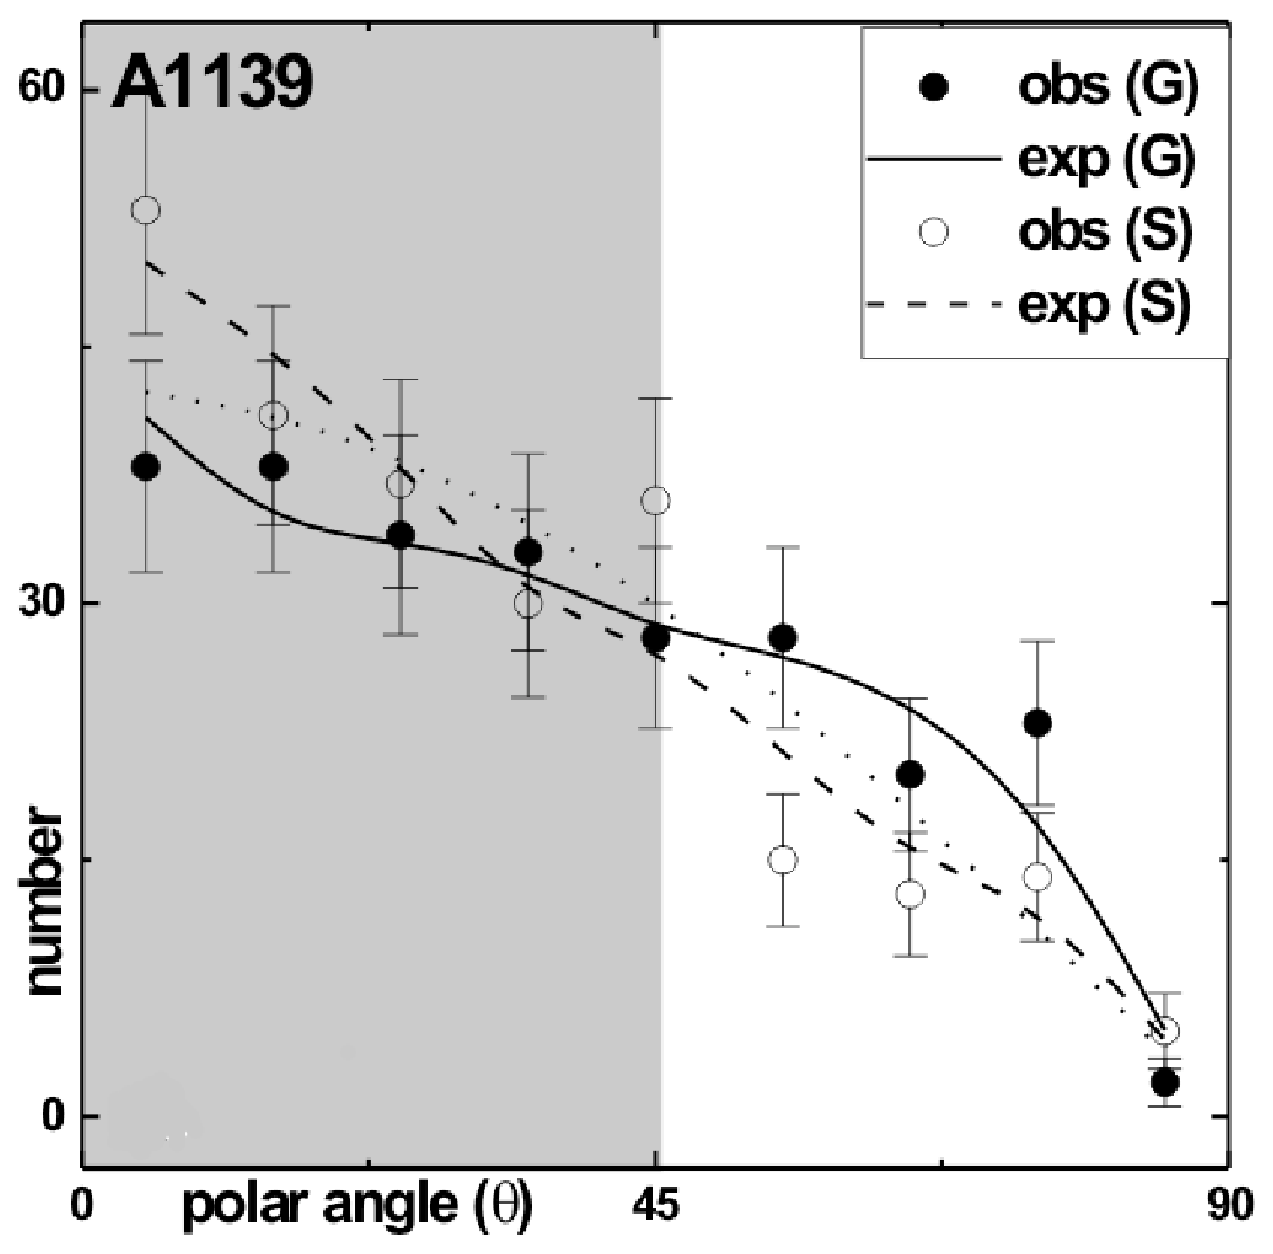
\includegraphics[height=6.9cm]{A1139_theta.eps}
      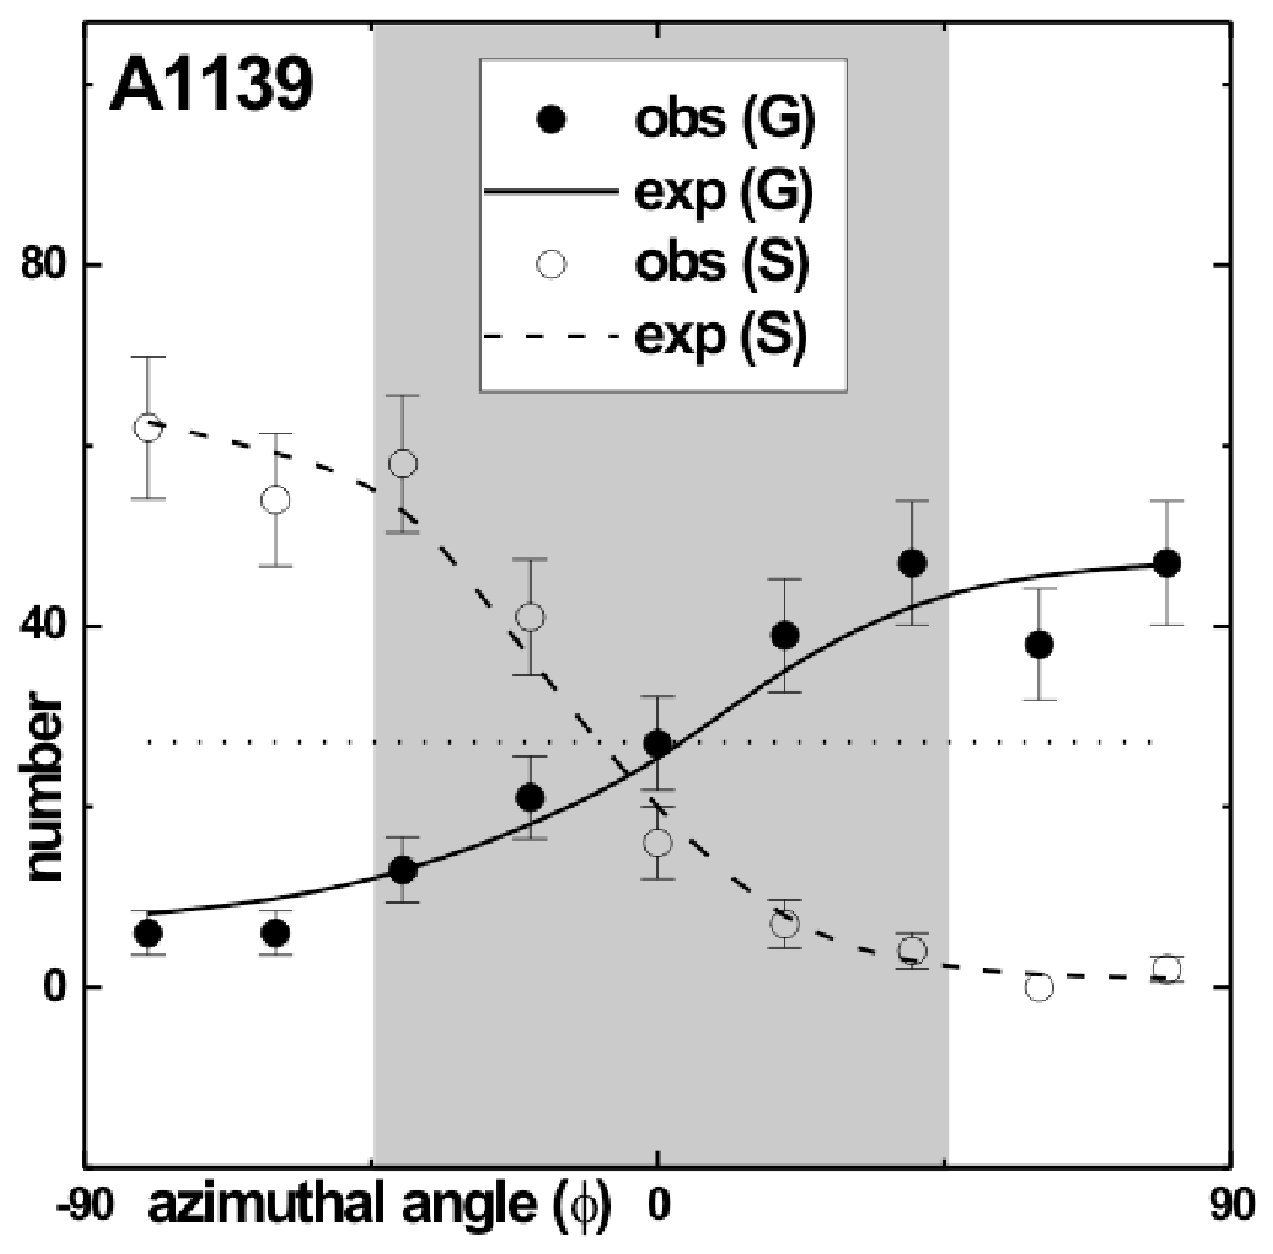
\includegraphics[height=6.9cm]{A1139_phi.eps}
            \caption[]{ The polar (left) and azimuthal angle (right) distributions of galaxies in A1139
with respect to the G (solid line) and S (dashed line) coordinate systems.
For comparison, cosine and average distributions (dotted line) are shown.
The polar angle, $\theta$ = 0$^\circ$ (90$^\circ$ ) corresponds to the galactic SV tends to lie
parallel (perpendicular) to the galactic/Supergalactic plane. The azimuthal
angle, $\phi$ = 0$^\circ$ means the direction to the galactic/Supergalactic centre. The
statistical error ($\pm\, 1\, \sigma$ ) bars are shown for the observed counts. A hump in the
grey-shaded region represents the SV of galaxies tend to lie in the reference
plane (left) and SV projections of galaxies tend to be directed towards the
centre of the reference coordinate system (right).
}
\end{figure}
\noindent All the statistical test support isotropy (see Table 5.1)
in both the $\theta$ and $\phi$ distributions suggesting a random orientation of spin vectors and spin vector projections of galaxies with respect to both galactic and Supergalactic coordinate systems. No significant humps and dips can be seen in the histogram. Our result supports the hierarchy model (Peeble 1969) in which galaxies were believed to be first formed and while they obtained angular momentum by tidal forces while they were gathering gravitationally to form clusters.\\\\
Strong isotropy in the spatial orientation of spin vectors of galaxies indicate that a single cluster in rotation rather than two overlapping clusters that either merge or depart from each other as pointed in Burgertt et al. (2004).
\subsection{Abell 2162}
Abell 2162 is one of the nearest cluster in our sample and is a member cluster in the Hercules Supercluser (Einasto et al. 2001). Neither a distinct substructure nor a significant local density peaks is found except for the cluster center. HL calculated rotational amplitude and global velocity gradient using the galaxies at inner region ($<18^\prime$, as the radial distribution was discontinuous at $\sim 18^\prime$) and found ${|v_{rot}|}/{\sigma_p}= 0.64$ and $\frac{dv}{dR}$=635, satisfying the criteria for rotating clusters.
\begin{figure}[H]
\centering
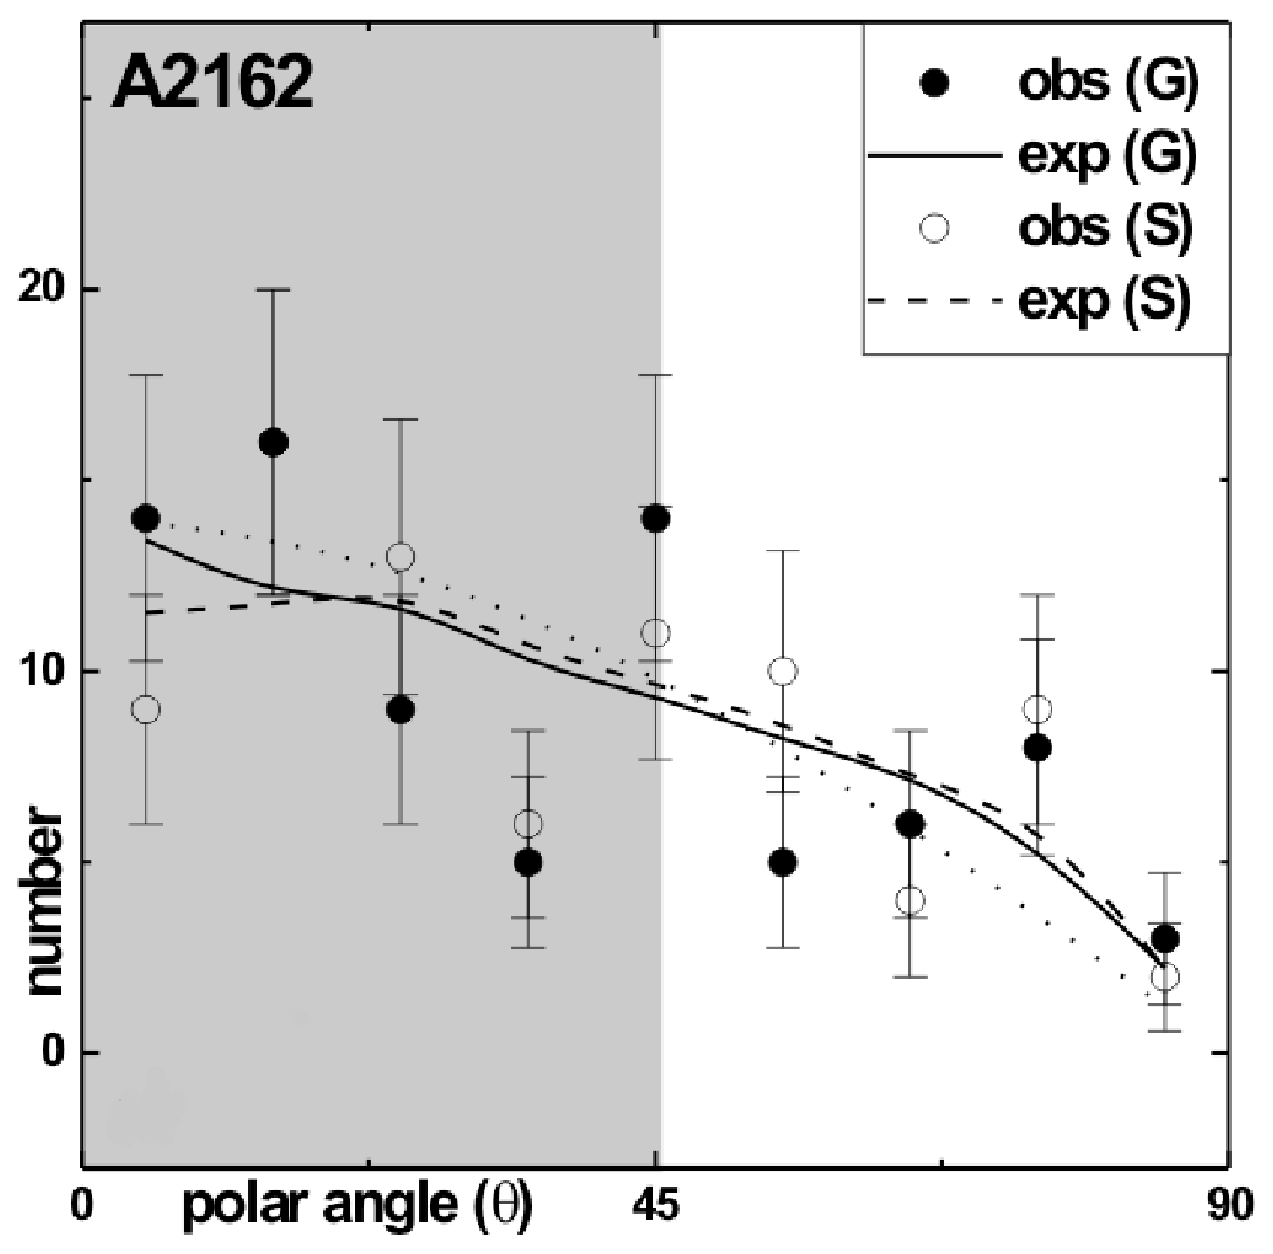
\includegraphics[height=6.9cm]{A2162_theta.eps}
   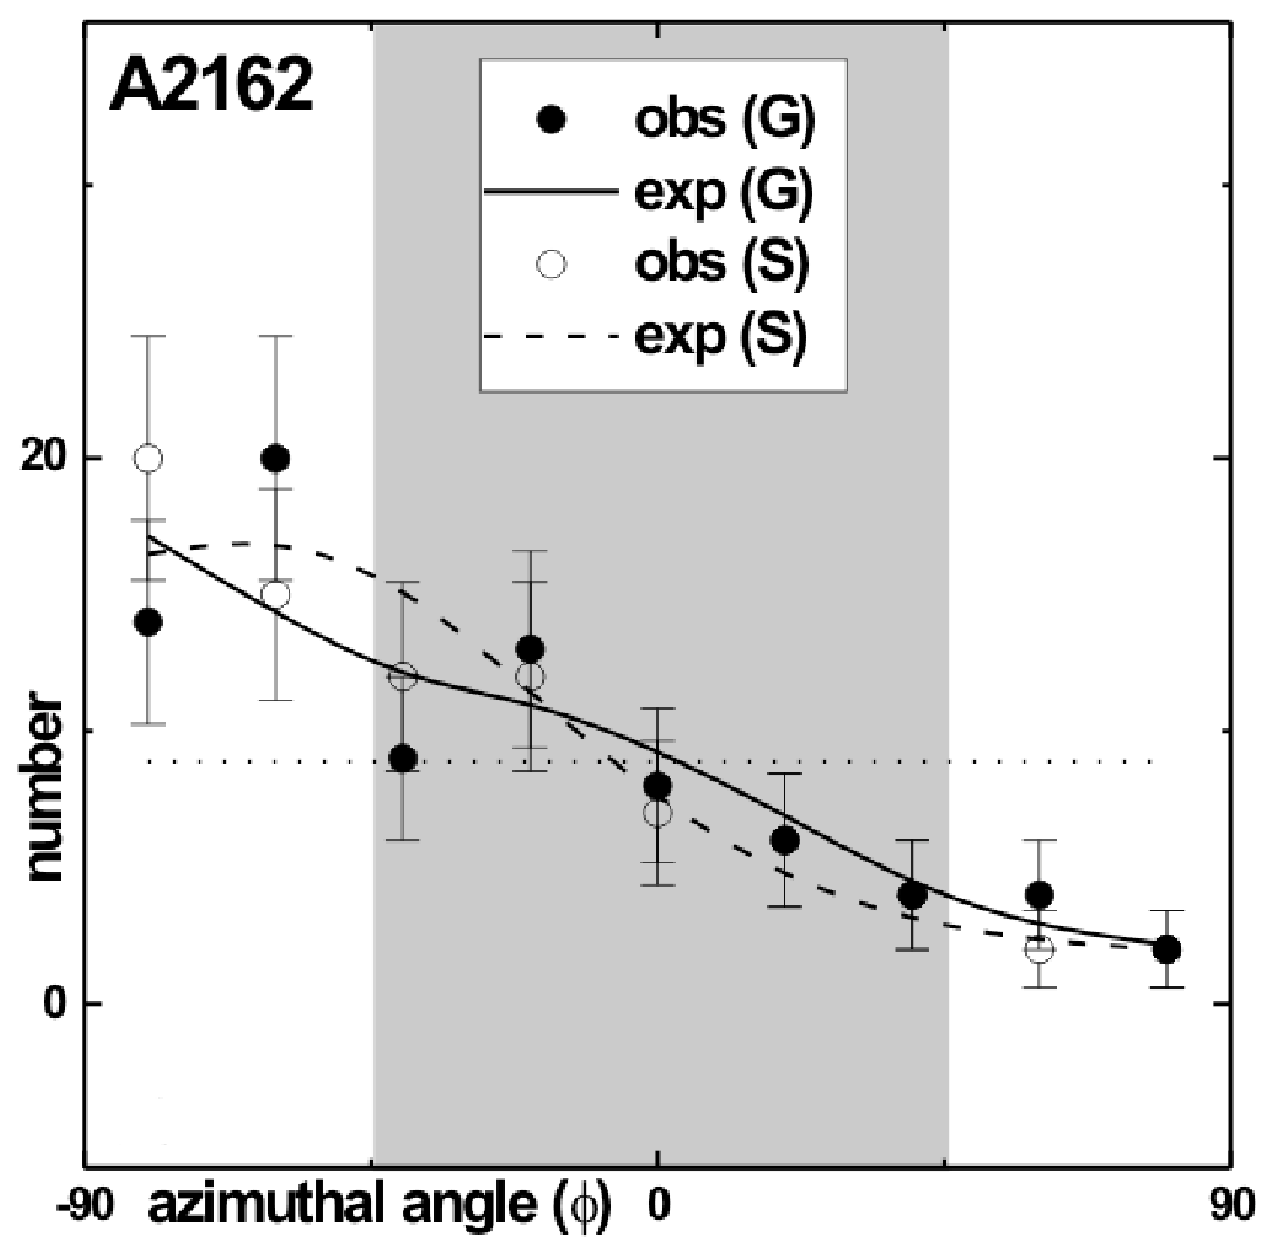
\includegraphics[height=6.9cm]{A2162_phi.eps}
      \caption{The polar (left) and azimuthal angle (right) distributions of galaxies in A2162
with respect to the G (solid line) and S (dashed line) coordinate systems.
For comparison, cosine and average distributions (dotted line) are shown.
The polar angle, $\theta$ = 0$^\circ$ (90$^\circ$ ) corresponds to the galactic SV tends to lie
parallel (perpendicular) to the galactic/Supergalactic plane. The azimuthal
angle, $\phi$ = 0$^\circ$ means the direction to the galactic/Supergalactic centre. The
statistical error ($\pm\, 1\, \sigma$ ) bars are shown for the observed counts. A hump in the
grey-shaded region represents the SV of galaxies tend to lie in the reference
plane (left) and SV projections of galaxies tend to be directed towards the
centre of the reference coordinate system (right).}
\end{figure}

\noindent A hump at $45^\circ$ and two dips at angle $35^\circ$ and $55^\circ$ can be seen in $\theta$ distribution. These humps and dips compensate each other and hence all statistical tests show isotropy (see Table 5.1). The binning effect cannot be ruled out here. Thus, no preferred alignment of spin vectors of galaxies with respect to both galactic and Supergalactic coordinate system is found. In the $\phi$ distribution, all statistical tests advocate isotropy. There is a very good agreement between the observed and expected distribution suggesting random orientation of spin vector projections of galaxies with respect to galactic and Virgo cluster center. Thus there is a good agreement between the hierarchy model and global rotation with the vanishing angular momentum is observed, suggesting the existence of Li model (Li 1998).

\subsection{Abell 2366} Jones \& Forman (1999) and Flin \& Krywult (2006) found no substructure using Einstein X-ray images and positional information of galaxies. Similarly, HL studied galaxy number density map and found no evidence of substructure, but a significant value of velocity dispersion. A weak bimodal velocity distribution with a large dispersion but weak central aggregration of galaxies was found. HL found ${|v_{rot}|}/{\sigma_p}= 0.57$ and $\frac{dv}{dR}$=788, satisfying the criteria for rotating clusters. So, they selected this as a probable rotating galaxy cluster.
\begin{figure}[H]
\centering
 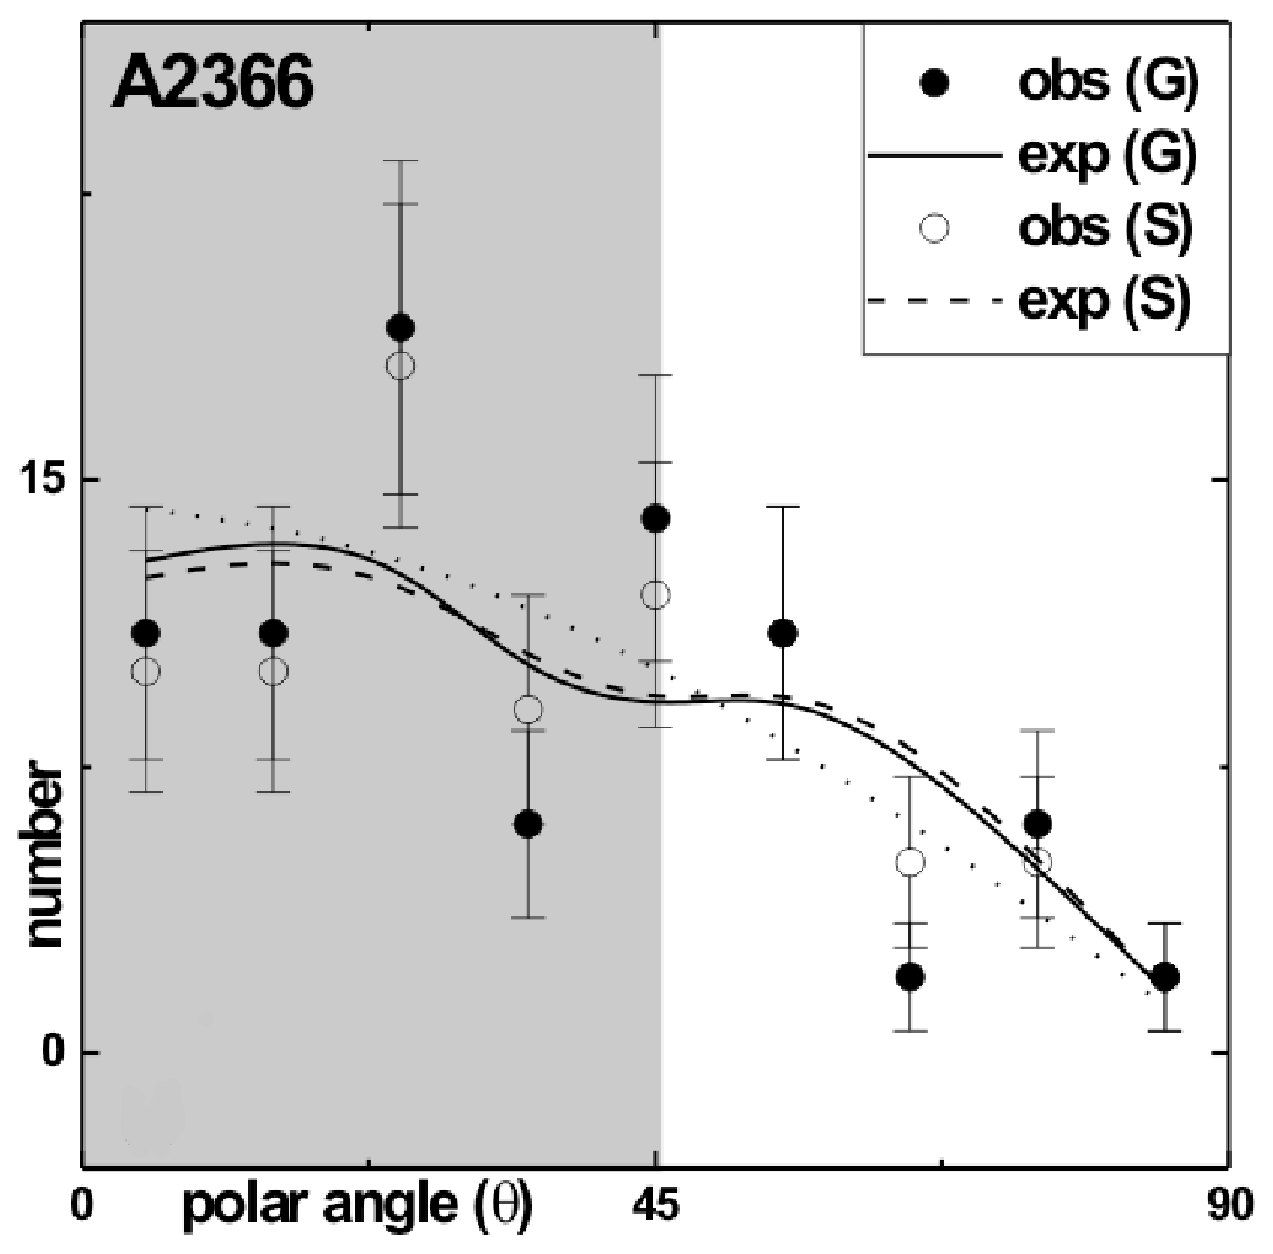
\includegraphics[height=6.9cm]{A2366_theta.eps}
   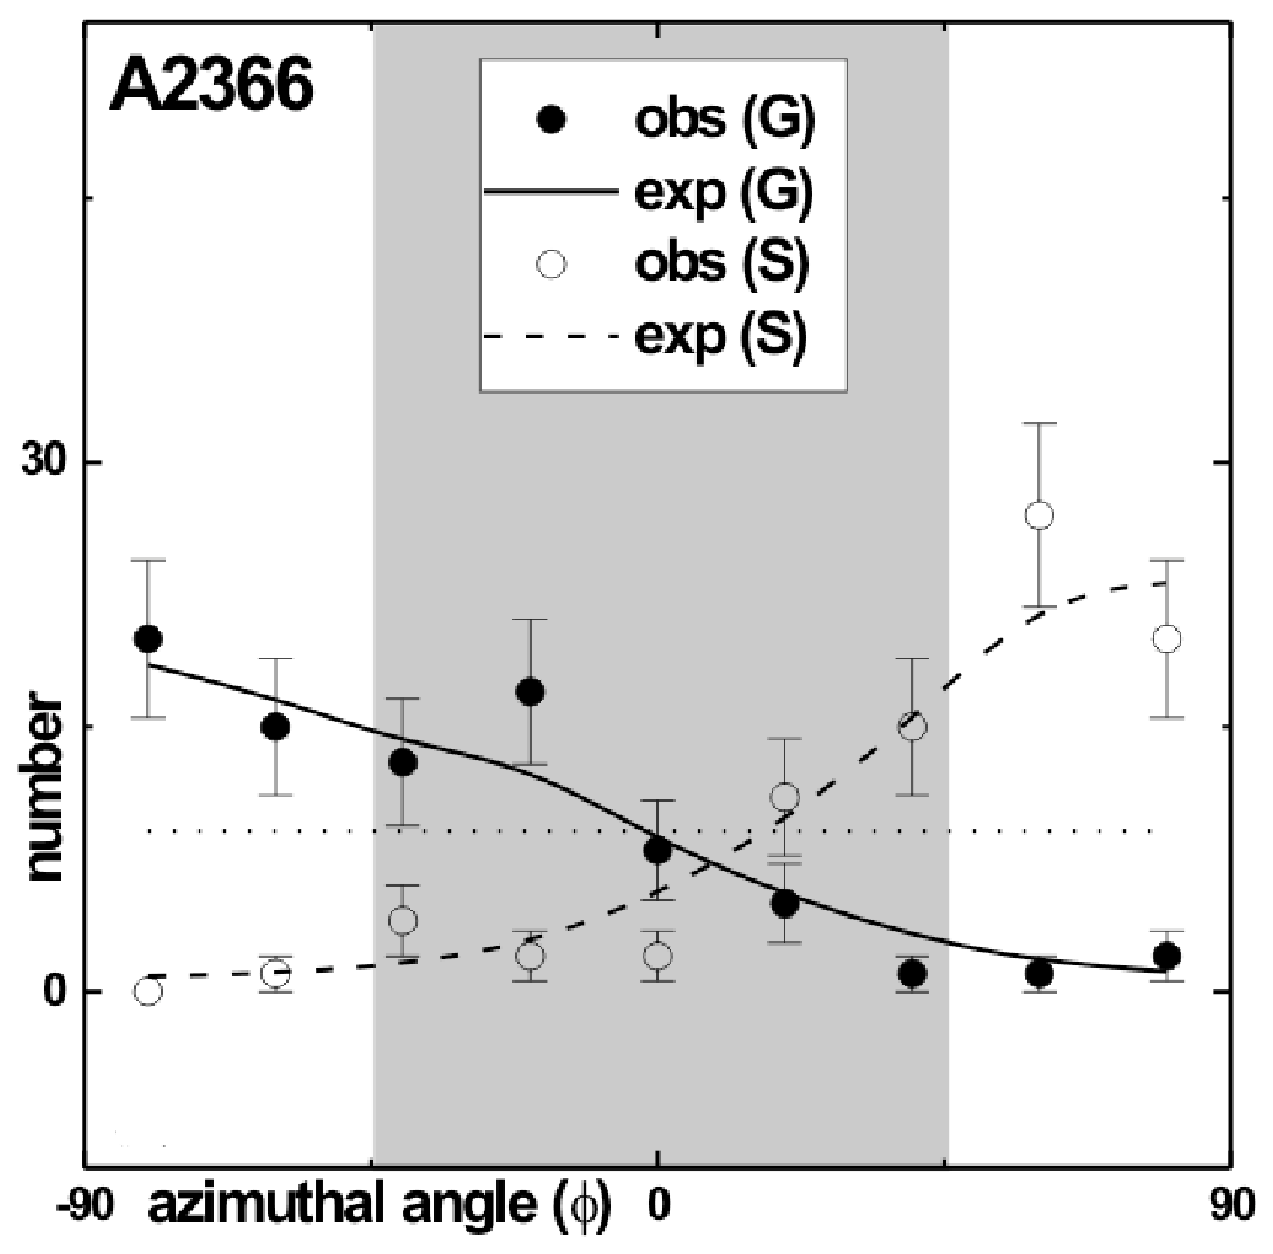
\includegraphics[height=6.9cm]{A2366_phi.eps}
     \caption{The polar (left) and azimuthal angle (right) distributions of galaxies in A2366
with respect to the G (solid line) and S (dashed line) coordinate systems.
For comparison, cosine and average distributions (dotted line) are shown.
The polar angle, $\theta$ = 0$^\circ$ (90$^\circ$ ) corresponds to the galactic SV tends to lie
parallel (perpendicular) to the galactic/Supergalactic plane. The azimuthal
angle, $\phi$ = 0$^\circ$ means the direction to the galactic/Supergalactic centre. The
statistical error ($\pm\, 1\, \sigma$ ) bars are shown for the observed counts. A hump in the
grey-shaded region represents the SV of galaxies tend to lie in the reference
plane (left) and SV projections of galaxies tend to be directed towards the
centre of the reference coordinate system (right).}
   
\end{figure}

\noindent A significant hump at $25^\circ$ followed by two dips at $35^\circ$ and $65^\circ$ can be seen in the spin vector distribution of member galaxies. These hump and dips compensate each other to show isotropy in the statistical test (see Table 5.1). A local effect can  not be ruled out here, probably due to the gravitational tidal forces due to the massive central region. In azimuthal angle distribution, a random orientation is observed in the statisitics as well as in histogram. Thus, it is found that the rotating cluster which is the dynamical equilibrium shows vanishing angular momentum as predicted by Godlowski et al. (2003) and observationaly verified by Godlwoski (2012).
\section{General Discussion}
\begin{figure}[H]
\centering
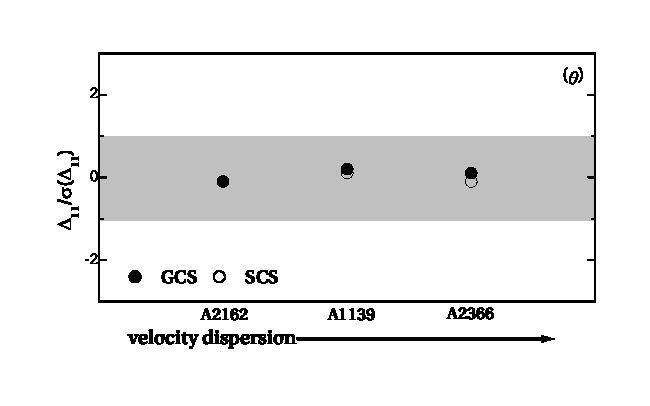
\includegraphics[height=6.9cm]{polar.eps}\\
 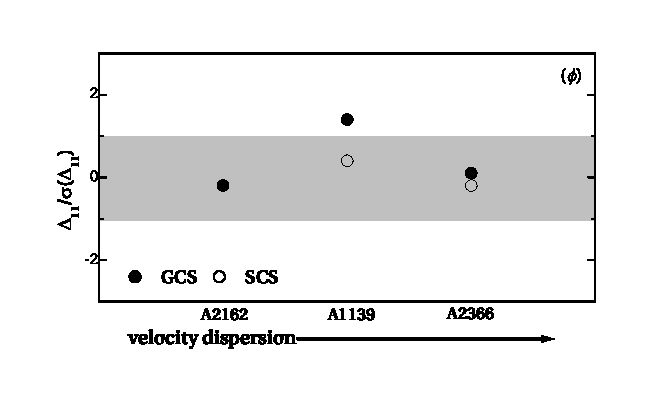
\includegraphics[height=6.9cm]{phi.eps}
     \caption{The orientation parameter (the First Order Fourier coefficient,  $\Delta_{11}$/$\sigma(\Delta_{11})$) plot for polar angle i.e. $\theta$ (top) and azimuthal angle i.e. $\phi$  (bottom) for three clusters with respect to the galactic and Supergalactic coordinate system. The region of isotropy is given by the shaded portion in graph.
-$1\leq\Delta_{11}$ /$\sigma(\Delta_{11})\leq +1$ for the isotropy and $\Delta_{11}/\sigma(\Delta_{11}) > \pm 1$ for anisotropy.} 
\end{figure}
\noindent From the Table 5.1 we can easily see that almost all statistical test supports isotropy of the distribution of the spin vectors of galaxy i.e. statistics supports hierarchy model. However, the first order Fourier coefficient test support anisotropy for the azimuthal angle distribution for the A1139 in galactic coordinate system. The polar angle distribution shows strong isotropy in both galactic and Supergalactic system. In case of azimuthal distribution, all the galaxies shows isotropy in Supergalactic coordinate system.\\\\
As the sign of $\Delta_{11}$ for the polar angle distribution gives the tendency of orientation  of spin vectors parallel or perpendicular to the plane of the reference coordinate system. i.e positive (negative) $\Delta_{11}$ suggests that spin vectors of galaxies tend to orient parallel (perpendicular) with respect to reference coordinate sysem. From figure 5.4 we can see angular momentum vectors of A1139 and A2366 tend to orient perpendicular to the reference plane of the galactic coordinate system but A2162 has the spin vector orientation parallel to the reference plane of the galactic coordinage system. However in case of Supergalactic coordinate system A2162 and A2366 tend to orient its angular momentum vector parallel to the plane but A1139 tend to orient it perpendicular to the plane of Supergalactic coordinate system.\\\\
The database, selection criteria, result and references of the published paper in MNRAS based on result of these three clusters (A1139, A2162, A2366) along with the result of other three clusters (A0954, A1399, A2169), which was proposed by HL as rotating clusters, is given in tabular form below:
\begin{center}
\begin{tabular}[lp=7cm]{|l|l|l|l|}
\hline\hline
Database&Selection&Results&References\\
&criteria&&\\
\hline
6 rotating&SDSS \& &- a random orientation of&Aryal,\\
clusters&2dFGRS&angular momentum vectors of&Bhattarai,\\
&database:&galaxies are found in all six&Dhakal,\\
&A954, A1139,&rotating clusters&Rajbahak \&\\
&A1399, A2162&supporting Hierarchy&Saurer\\
&A2169, and&model of galaxy&(2013)\\
&A2366&formation&\\
&&-It is found that the vanishing&\\
&&angular momentum is preferred by&\\
&&the rotating clusters which are in&\\
&&dynamical equilibrium and&\\
&&have large value of&\\
&&velocity dispersion&\\
\hline
\end{tabular}
\end{center}


